%18/11 - Dido Carrero
\part{Variantes genómicas: técnicas, llamada de variantes y anotación}
\chapter{Introducción a las variantes germinales}
\section{Análisis genómico}
El análisis genómico incluye varios pasos: primero, la extracción de muestras y la preparación de las librerías; luego, la secuenciación, el control de calidad de los archivos FastQ (donde se descartan las lecturas con errores, ya que una mayor refinación del pipeline implica un control de calidad más estricto); el alineamiento de las lecturas; la identificación o llamada de variantes (SNP, INDEL, CNV, SV); la anotación de los archivos VCF; la visualización de las variantes candidatas y, finalmente, los pasos de priorización y filtrado.

En general, en un análisis de genoma, pueden encontrarse muchas variantes en comparación con el genoma de referencia, por lo que es necesario aplicar filtros para identificar aquellas que sean realmente relevantes a nivel clínico. La validación final se realiza en el laboratorio mediante PCR.

Las variantes germinales se originan en la línea germinal, es decir, en los gametos, lo que las hace heredables y presentes en todo el organismo. En cambio, las variantes somáticas ocurren en células que no pertenecen a los gametos, son mutaciones adquiridas durante la vida y afectan solo a un linaje celular específico.

En la práctica, ya sea que se realice un análisis somático o germinal, se extraen muestras tanto del tejido tumoral como del tejido sano. Si se sospecha de una enfermedad genética germinal, también se debe extraer una muestra de un tejido germinal.

La frecuencia alélica es la proporción de moléculas de ADN en la muestra que contienen una mutación específica. Se calcula mediante la siguiente fórmula:
$$VAF = \frac{sequence.reads.with.a.DNA.variant}{overall.coverage.at.that.locus}$$
Este número es clave para diferenciar una variante somática de una germinal. En un organismo diploide, un locus heterocigoto debería mostrar un VAF cercano a 0,5, un locus homocigoto tendrá un VAF de 1 y un locus de referencia tendrá un VAF de 0. Las variantes somáticas presentan una frecuencia alélica muy variable, mientras que las variantes germinales suelen tener valores de VAF de 0, 0,5 o 1, dependiendo de si están presentes en uno, ambos o ninguno de los alelos.

\subsection{GATK}
GATK es un conjunto de herramientas desarrollado por el Broad Institute para el análisis de variantes genómicas. A partir de archivos BAM, estas herramientas permiten realizar un análisis completo de variantes. El paquete incluye buenas prácticas y un flujo de trabajo (workflow) que varía dependiendo de si se analizan variantes germinales o somáticas.

\begin{figure}[h!]
\centering
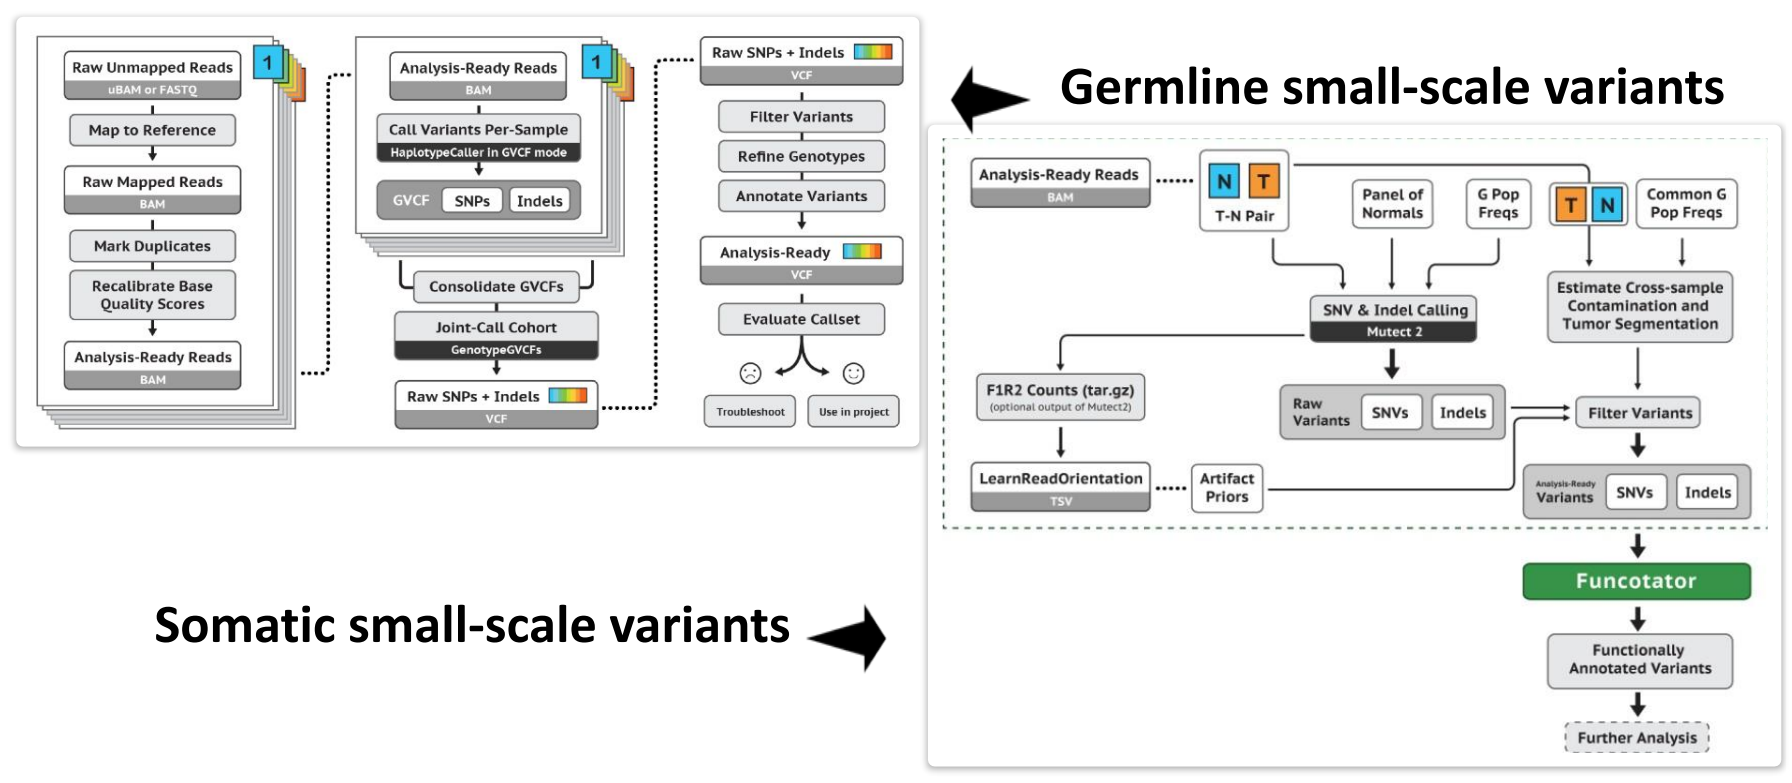
\includegraphics[width = 0.8\textwidth]{figs/gatk-pipelines.png}
\end{figure}

HaplotypeCaller es una herramienta utilizada para la llamada de variantes, basándose en el cálculo de la probabilidad de los genotipos. Utiliza un archivo BAM como entrada y produce un archivo de salida en formato VCF o GVCF con los genotipos 1/1, 0/1 y 0/0. Este archivo VCF debe ser filtrado mediante recalibración de bases (una práctica recomendada) o mediante hard-filtering. Si el archivo de salida es un GVCF, será necesario realizar un paso intermedio antes de aplicar el filtro y continuar con el análisis posterior. Además, con la opción -ploidy, se puede especificar la ploidía del organismo.

El comando básico para la herramienta es:
\begin{lstlisting}[language = bash]
gatk HaplotypeCaller \
	-R reference.fasta \
	-I preprocessed_reads.bam \
	-O germline_variants.vcf
\end{lstlisting}

MuTect2 es una herramienta diseñada para la llamada de variantes somáticas. Permite detectar SNVs e INDELs, con frecuencias alélicas variables, y es capaz de diferenciar entre variantes somáticas y germinales. MuTect2 ofrece varios modos: tumor con normal emparejado, solo tumor o modo mitocondrial.

\section{Práctica: análisis de datos}
Vamos a recibir los datos de cáncer de mama. Se ha secuenciado todo el exoma con Illumina. Primero creamos el entorno conda \texttt{OVCA\_case}. 
\begin{lstlisting}[language=bash]
conda create -n OVCA_case
conda activate OVCA_case
conda install bioconda::gatk4
conda install bioconda::samtools
\end{lstlisting}

Con los datos descargados, utilizamos la herramienta HaplotypeCaller. Lo primero que debemos hacer es realizar los índices de la referencia y del fichero bam:
\begin{lstlisting}[language=bash]
samtools dict  REFERENCE/hg19_chr17.fa -o  REFERENCE/hg19_chr17.dict
samtools faidx REFERENCE/hg19_chr17.fa
samtools index bams/normal_refined.bam
\end{lstlisting}

A continuación utilizamos la herramienta:
\begin{lstlisting}[language=bash]
gatk HaplotypeCaller -R REFERENCE/hg19_chr17.fa -I bams/normal_refined.bam -O out/normal_refined_out.vcf
\end{lstlisting}

El fichero resultante empieza con una cabecera con dos almohadillas y el cromosoma de referencia. Se muestra la información acerca de la generación del fichero y los filtros. Con una almohadilla se muestra el significado de cada columna: cromosoma en el que está la variante, posición genómica, ID, alelo de referencia, alelo alternativo con la mutación encontrada, score de calidad, filtros, información adicional con la anotación, formato del siguiente campo y normal. Dentro del formato, se distinguen: GT indica el genotipo, AD el número de lecturas que soporta la variante (en formato referencia,variante) y DP el total de lecturas.

El siguiente paso es la recalibración de variantes. Muchas veces, la calidad de las variantes que aparece de manera directa (columna QUAL) se debe recalibrar. Este modelo puntúa las calidades de las variantes y filtrar aquellas que no pasen los filtros. Se comprueba que una variante sea efectivamente verdadera. Para ello, se da un archivo de referencia de variantes y se estima si la variante es un artefacto de la secuenciación o una variante de verdad. El resultado es VQSLOD, que se añade al campo de información. Esto en general se realiza para SNPs e INDELs por separado debido a que las bases de datos de variantes son diferentes. 

El paso siguiente es aplicar los filtros VQSR. En la columna FILTER anota si la variante pasa filtros o no, pero no descarta aquellos que no pasen los filtros; si se quiere eso se debe especificar.
\begin{lstlisting}[language=bash]
tabix -p vcf Annotations/dbsnp_138.hg19_chr17.vcf.gz

gatk VariantRecalibrator -R REFERENCE/hg19_chr17.fa -V out/normal_refined_out.vcf
--resource:dbsnp,known=true,training=true,truth=true,prior=15.0
Annotations/dbsnp_138.hg19_chr17.vcf.gz -an QD -an ReadPosRankSum -an FS -an SOR -mode BOTH -O out/output_normal_refined.recal --tranches-file out/output_normal_refined.tranches

gatk ApplyVQSR -R REFERENCE/hg19_chr17.fa -V out/normal_refined_out.vcf -O out/output_normal_refined.recalibrated --truth-sensitivity-filter-level 99.0 --tranches-file out/output_normal_refined.tranches --recal-file out/output_normal_refined.recal -mode BOTH
\end{lstlisting}

El último paso es el filtrado de las variantes. 
\begin{lstlisting}[language=bash]
awk -F '\t' '{if ($0 ~ /#/ || $7 == "PASS") print}' out/output_normal_refined.recalibrated > out/output_normal_refined.onlypass

#Contar el número de líneas resultantes
grep "^chr17" out/output_normal_refined.onlypass | wc -l
\end{lstlisting}

%21/11 - Dido
\chapter{Introducción a las variantes somáticas}
\section{Control de calidad y refinamiento de alineamientos}
\subsection{Control de calidad}
Los controles de calidad se suelen hacer en varios puntos de todo el proceso. Hay varios puntos clave, y después de cada uno de ellos se realiza el control de calidad. El primero y más importante parte de los archivos FastQ de secuenciación, ya que si éstos están mal, el resto del análisis carece de sentido.

Se utiliza el programa FastQC que da un informe en HTML con varias estadísticas de los archivos. Hay otros programas que se pueden utilizar, como samtools, que indica si hay secuencias duplicadas y otras estadísticas. MultiQC combina varias herramientas para sacar un informe completo.

En los controles de calidad, se mira si hay un número de lecturas dentro del rango esperado, si las bases tienen una buena calidad mediante el Phred score, y si hay contaminación en las muestras. Una secuencia que aparezca repetidamente puede ser muy repetitiva en el genoma que se secuencie o una contaminación.

FastQC permite visualizar la calidad por base por secuencia, el contenido GC y secuencias sobrerrepresentadas entre otras métricas, pero esas son las que habitualmente están mal. En cuanto a la evaluación de la calidad por base, se ve la distribución de los scores en las lecturas. En secuenciación de Illumina, es habitual que al final de las lecturas la calidad decaiga un poco, pero debería seguir en un rango elevado. Si la calidad decae mucho, se trata de un error en la secuenciación. En los scores por secuencia, se espera que la mayoría de las secuencias tengan una puntuación muy alta. Si hay varias secuencias con una calidad baja, eso indica que algo está mal, pero es difícil indicar la causa (problema del secuenciador, purificación de las muestras, contaminación, librería, etc). La distribución esperada del contenido en GC debería seguir una distribución normal, aunque hay veces que se puede desviar un poco.

\begin{lstlisting}[language=bash]
conda install bioconda::fastqc
fastqc -o out/ Raw_data/*.fastq
\end{lstlisting}

El resultado es un fichero html y zip por cada FastQ. En cuanto a Normal R1, el contenido GC muestra un mensaje de error. Hay un pico muy grande alrededor del 60\%, cuando en humanos debería rondar el 50\%. Además, hay varias lecturas con un contenido GC bajo, sobre el 35\%. Como estos resultados son malos, se puede valorar descartarlos y repetir la secuenciación, pero en laboratorios pequeños puede ser un problema. Además, tenemos una secuencia sobrerrepresentada de N, que no nos preocupa porque se va a descargar. Todas las demás métricas han salido bien. En Normal R2, las secuencias sobrerrepresentadas dan error, pero sigue siendo una secuencia de todo N, por lo que se le puede dar poca importancia. El contenido GC también da error. En cuanto a las muestras de tumor, son muy similares: tienen un contenido GC más bajo y tiene una secuencia de N sobrerrepresentada. 
Hay que tener en cuenta que estamos trabajando solo con el cromosoma 17, pero que la distribución esperada está calculada sobre todo el genoma. Por tanto, si ese cromosoma tiene muchas secuencias repetitivas en AT, ya de por sí habrá un sesgo en la comparación con la distribución esperada. 

\subsection{Alineamiento}
En cuanto al alineamiento, se utiliza BWA. Se puede utilizar la siguiente chuleta para la indexación en base al fichero que se tenga:
\begin{lstlisting}[language=bash]
#Fasta
bwa index reference.fasta
samtools dict reference.fasta -o reference.dict
samtools faidx reference.fasta

#BAM
samtools index bam.file

#VCF
tabix -p vcf vcf.file
\end{lstlisting}

El siguiente paso es la alineación.
\begin{lstlisting}[language=bash]
bwa mem -R '@RG\tID:OVCA\tSM:Normal' REFRENCE/hg19_chr17.fa Raw_data/WEx_Normal_R1.fastq Raw_data/WEx_Normal_R2.fastq > alignment/normal.sam
bwa mem -R '@RG\tID:OVCA\tSM:Tumour' REFRENCE/hg19_chr17.fa Raw_data/WEx_Tumour_R1.fastq Raw_data/WEx_Tumour_R2.fastq > alignment/tumour.sam
\end{lstlisting}

Se puede utilizar \texttt{samtools flagstat normal.sam} para ver unas estadísticas como alineamientos mapeados, primarios, secundarios, duplicados, etc. 

\subsection{Refinamiento del alineamiento}
En este paso, queremos convertir los SAM en BAM para que los ficheros estén comprimidos y binarizados. Además, BWA a veces omite alguna información en los ficheros SAM que queremos rellenar.
\begin{lstlisting}[language=bash]
samtools fixmate -O bam alignment/normal.sam alignment/normal_fixmate.bam
samtools fixmate -O bam alignment/tumour.sam alignment/tumour_fixmate.bam
\end{lstlisting}

Los duplicados vienen de la amplificación por PCR durante la preparación de la librería. Un error al principio de la PCR se propaga. Los duplicados en secuenciación híbrida no aportan nada al análisis posterior, pudiendo dar lugar a falsos positivos y redundancia. Por ello, lo mejor es descartar estas duplicaciones. Además, para la llamada de variantes es necesario que el alineamiento esté ordenado por posición genómica, y aprovechamos para indexar el BAM.
\begin{lstlisting}[language=bash]
samtools sort -O bam -o alignment/normal_sorted.bam alignment/normal_fixmate.bam
samtools sort -O bam -o alignment/tumour_sorted.bam alignment/tumour_fixmate.bam

samtools rmdup -S alignment/normal_sorted.bam alignment/normal_refined.bam
samtools rmdup -S alignment/tumour_sorted.bam alignment/tumour_refined.bam

samtools index alignment/normal_refined.bam
samtools index alignment/tumour_refined.bam
\end{lstlisting}

Con esto hemos creado los bams que utilizamos en la parte anterior de las variantes germinales. Se pueden eliminar los ficheros intermedios de ficheros sam, fixmate y sorted, dejando los bam refinados.

\section{Recalibración de la calidad de base}
Cada posición de la secuencia tiene su calidad de base. Las diferentes tecnologías NGS tienen sus sesgos dependiendo del contexto, por lo que es importante hacer la recalibración para corregir empíricamente esos sesgos. La recalibración de bases no es lo mismo que la recalibración de variantes (eso viene después con los VCF).

La recalibración de bases consta de dos pasos. Primero, BaseRecalibrator parsea las lecturas y crea una tabla en la que se asigna a cada lectura el ciclo durante el que se leyó la base, su puntuación y la puntuación de las bases que van antes y después. EL modelo computa cuántas veces hay un cambio en la referencia según dbSNP, excluyendo los loci de alta variabilidad. Después, la herramienta ApplyBQSR parsea las lecturas y, utilizando la matriz de antes, recalibra las puntuaciones. Así, las calidades son más similares a las puntuaciones empíricas, pudiendo utilizarse para el variant calling.

\section{Llamada de variantes somáticas}
Las variantes son cambios permanentes en el ADN de un organismo que pueden deberse a errores durante la replicación, durante la recombinación durante la formación de gametos y por factores externos como radiación, viruses, transposones, rayos ultravioleta, etc. El genoma entre humanos es idéntico en un 99,9\%. El 0,1\% restante es la fuente de variabilidad, permitiendo los mecanismos de evolución, las diferencias fenotípicas entre individuos y en la respuesta a enfermedades y fármacos. 

\begin{figure}[htbp]
\centering
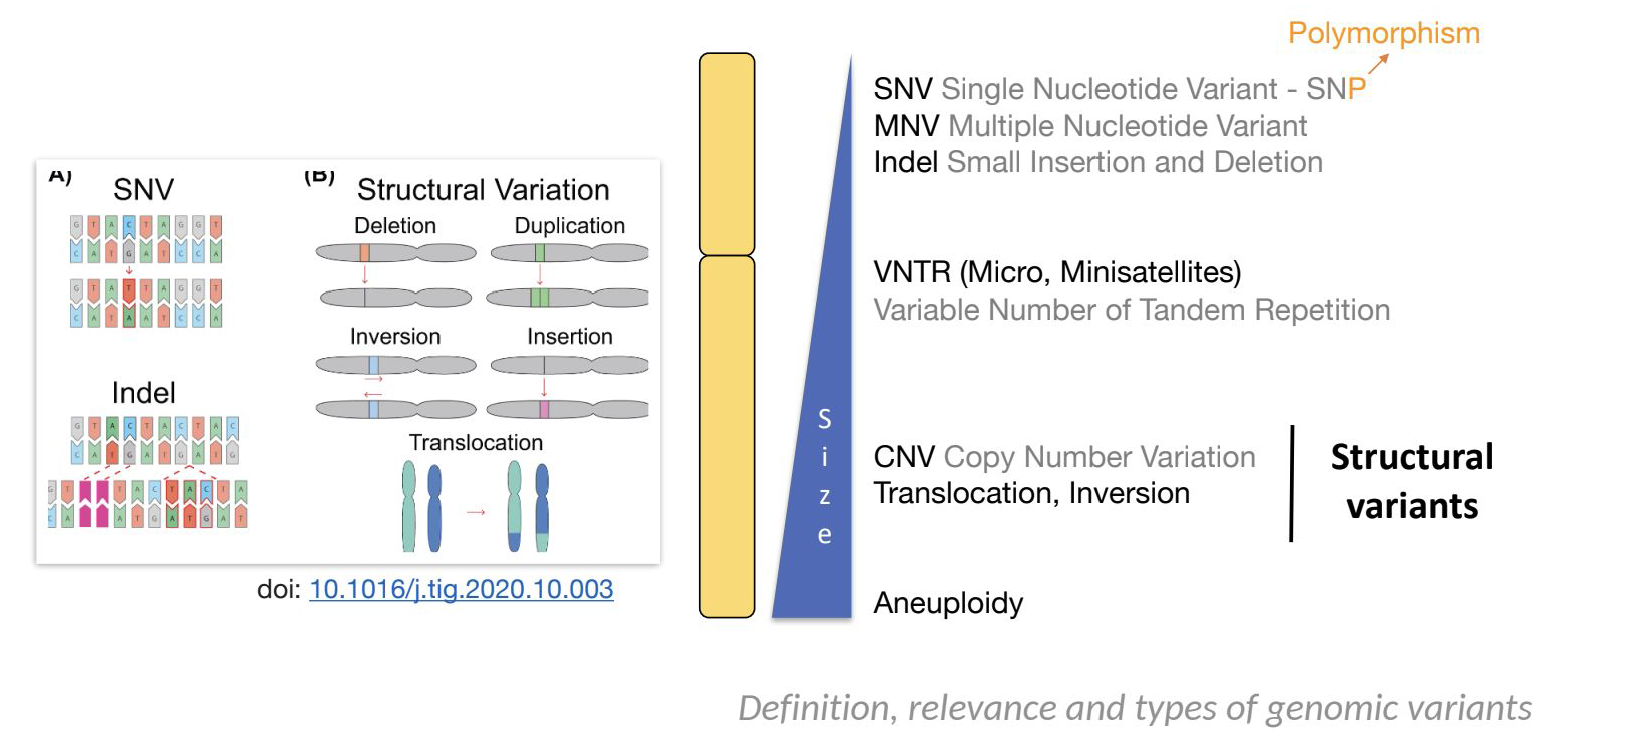
\includegraphics[width = \textwidth]{figs/variants-size.png}
\end{figure}

En función de la posición de la secuencia, puede haber variantes intergénicas (entre genes) en secuencias reguladoras o upstream o downstream de algún gen en concreto. Dentro de genes, puede haber variantes en las regiones UTR, en los exones, en los intrones o en regiones de splicing. 

Para realizar la llamada de variantes, se utiliza MuTect2. Es similar a GATK, pero permitiendo mayor variabilidad de frecuencia alélica (no solo 0, 0,5 y 1 como GATK), además de evitar las variantes germinales. Hay distintos modos: tumor con tejido normal (este es el óptimo), solo tumor y mitocondrial. Se crea un panel de normales para poder inferir qué mutaciones son exclusivamente somáticas. 
\begin{lstlisting}[language=bash]
#Modo Tumor-only 
gatk Mutect2 -R REFERENCE/hg19_chr17.fa -I alignment/tumour_refined.bam -O tumour_only_somatic.vcf

#Modo tumor with matched normal
gatk Mutect2 -R REFERENCE/hg19_chr17.fa -I alignmetn/tumour_refined.bam -I alignment/normal_refined.bam -normal Normal -O out/tumour_matched_somatic.vcf
\end{lstlisting}
 
Después del filtrado, obtenemos las siguientes variantes somáticas:
\begin{lstlisting}[language=bash]
grep "^chr17" out/tumour_matched_somatic.vcf | wc -l #193
grep "^chr17" out/tumour_only_somatic.vcf | wc -l #461
\end{lstlisting}
Cuando solo se mide el tumor, el número es casi el doble. Al dar el normal, el algoritmo sabe qué variantes son germinales por estar ya presentes en el tejido y los descarta. Al medir solo el tumor, algunas variantes germinales se excluyen, pero otras se cuelan, por lo que el número de variantes es mayor. 

Las frecuencias alélicas vienen en la columna FORMAT bajo AF. Estas frecuencias van del 0 al 1 en todo el rango. En las variantes germinales, esta información aparece en INFO y es de 0, 0,5 o 1. 

El fichero de solo tumor, tiene más variantes porque no puede excluir todas las variantes germinales. No obstante, el número de mutaciones sigue siendo mayor que la suma de tumor matched y las mutaciones germinales calculadas en la parte anterior. Esto se debe a que, al calcular las variantes germinales, el algoritmo solo se queda con aquellas que tengan una frecuencia alélica de 0,5 o de 1, no con todo el rango como el que detecta tumor only. Por ejemplo, por contaminación, tumor only puede detectar una variante germinal que no esté al 0,5 o 1 y que, por tanto, esté excluida del análisis de variantes germinales. El fichero de tumor only siempre va a  tener más variantes.

%25/11 - Dido
\chapter{Anotación de variantes}
La anotación de variantes consiste en enriquecer los archivos VCF con información adicional útil para su priorización. Esta información proviene tanto de bases de datos como de cálculos basados en la posición genómica de las variantes.

Dado el gran número de variantes en un archivo VCF, es impráctico evaluarlas manualmente. Como no todas tienen impacto relevante en el fenotipo de estudio, se aplican filtros para reducir el conjunto a las variantes potencialmente relevantes. Esto incluye descartar variantes comunes, benignas o de significancia incierta (VUS, variants of unknown significance).

En una anotación estándar, se incluye información sobre:
\begin{itemize}
\item Tipo de variante (SNV, indel, etc.)
\item Localización genómica
\item Consecuencias en la secuencia
\item Predicción del impacto funcional
\item Frecuencia poblacional
\item Asociación con patologías conocidas
\end{itemize}

\section{Nomenclatura de variantes}
Las variantes se identifican por el cromosoma, la coordenada genómica, el alelo de referencia y el alelo alternativo. Existen dos genomas de referencia principales: hg19 y hg38. El más reciente, hg38, es el recomendado para investigaciones actuales. Para convertir coordenadas entre estas referencias, se puede utilizar la herramienta Liftover disponible en UCSC.

El impacto en el ADN codificante y en la proteína se describe según la nomenclatura HGVS:
\begin{itemize}
\item g. genomic reference sequence
\item c. coding DNA reference sequence
\item m. mitochondrial DNA reference sequence
\item n. non-coding DNA reference sequence
\item r. RNA reference sequence (transcript)
\item p. protein reference sequence
\end{itemize}

Para asegurar la uniformidad, se recomienda seguir las \href{https://hgvs-nomenclature.org/stable/recommendations/general/}{guías estandarizadas para la nomenclatura HGVS}.

Las mutaciones pueden tener efectos diferentes en los transcritos de un mismo gen debido al splicing alternativo. Algunas enfermedades surgen por mutaciones que afectan transcritos minoritarios mientras que el principal permanece intacto. Para gestionar esta complejidad, se usan identificadores únicos, como los de Ensembl:
\begin{itemize}
\item Gene Identifiers: ENSG 
\item Transcript Identifiers: ENST
\end{itemize}

Además, las bases de datos como \href{https://www.genecards.org/}{GeneCards} o \href{https://www.genenames.org/}{GeneNames} ayudan a identificar el nombre oficial del gen, ya que un mismo gen puede tener varios nombres comunes.

Ensembl proporciona información detallada sobre cada gen, sus transcritos y biotipos, junto con equivalencias entre diferentes bases de datos. Por ejemplo:
\begin{itemize}
\item RefSeq incluye principalmente el transcrito principal
\item MANE es una anotación colaborativa que indica el transcrito principal
\end{itemize}

Para proteínas, la base de datos por referencia es \href{https://www.uniprot.org/}{Uniprot},  que incluye información sobre función, localización subcelular, relación con enfermedades y efectos de mutaciones.
Además, APPRIS (proyecto de Gencode) identifica transcritos principales y sus isoformas, categorizados como MANE, canonical o APPRIS principal.

\section{Consecuencias en la secuencia}
El impacto de una variante depende de su ubicación dentro del gen o región reguladora. Las consecuencias están codificadas y documentadas en \href{https://www.ensembl.org/info/genome/variation/prediction/predicted_data.html}{Ensembl}. 

\begin{figure}[htbp]
\centering
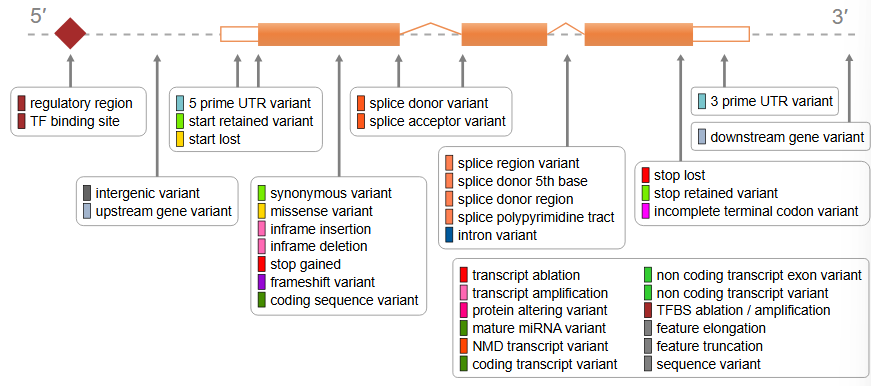
\includegraphics[width = \textwidth]{figs/consequences.png}
\end{figure}

\begin{itemize}
\item Mutaciones puntuales:
\begin{itemize}
\item Missense: cambian un aminoácido. Pueden ser conservativas o no conservativas en función de si mantienen la polaridad.
\item Nonsense: introducen un codón de parada
\item Silentes: no afectan al aminoácido
\end{itemize}
\item Mutaciones inframe: no alteran el marco de lectura
\item Mutaciones frameshift: cambian el marco de lectura, afectando significativamente la proteína.
\end{itemize}

Las consecuencias se clasifican según su impacto:
\begin{itemize}
\item Alto: frameshift, nonsense
\item Moderado: missense
\item Bajo: silentes
\item Modificador: sin efecto directo conocido
\end{itemize}

Esta clasificación facilita priorizar variantes según su potencial efecto dañino.

\section{Predicción del impacto funcional}
Existen numerosos algoritmos para predecir el impacto de variantes en la función y estructura de proteínas. Estos se agrupan en:
\begin{itemize}
\item Predictores para variantes missense
\item Predictores para variantes que afectan el splicing
\item Predictores basados en la conservación evolutiva
\end{itemize}

\subsection{Predictores para variantes missense}
El hecho de que haya tantos predictores hace que haya varias escalas para predecir el impacto de un cambio. Cada software tiene su escala y sus criterios para ver si una variante es benigna o no. Por ello, se realiza la anotación con varios y se busca el consenso entre ellos. Algunos predictores son:
\begin{itemize}
\item \textbf{Sift:} evalúa el efecto funcional basándose en homología y propiedades de aminoácidos. Score: 0-1 (más bajo = mayor impacto); < 0,05 deleterious
\item \textbf{PolyPhen:} basado en estructura y función proteica. Score: 0-1 (más alto = mayor impacto); benigno < $\sim$ 0,435 < dañino
\item \textbf{Revel:}  integra 13 herramientas, incluidas SIFT y PolyPhen, para una predicción más robusta.
\item \textbf{ClinPred:} utiliza machine learning para identificar variantes relevantes en enfermedades, incorporando frecuencias alélicas de gnomAD.
\item \textbf{AlphaMissense:} se trata de una adaptación de AlphaFold ajustada a bases de datos de frecuencias de poblaciones de variantes humanas y primates para predecir la patogenicidad de variantes sin sentido combinando el contexto estructural y la conservación evolutiva. Genera predicciones para todas las posibles sustituciones de aminoácidos en humanos y clasificación del 89\% de las variantes sin sentido como probablemente benignas o patógenas.
\end{itemize}

Como no hay consenso, a la hora de realizar la prioridad hay que tener en cuenta su score. Estos predictores tienen una precisión y especificidad moderada, por lo que se deben utilizar en conjunto y ver el consenso.

\subsection{Predictores para variantes de splicing}
En cuanto a los predictores de splicing, uno muy notable es \textbf{SpliceAI}. Se trata de una herramienta basada en deep-learning que identifica las variantes de splicing y predice el efecto. La puntuación delta de una variante oscila entre 0 y 1 y puede interpretarse como la probabilidad de que la variante altere el splicing. En el artículo se ofrece una caracterización detallada de los valores de corte de 0,2 (alta recuperación), 0,5 (recomendado) y 0,8 (alta precisión).

\section{Frecuencias poblacionales}
Las frecuencias poblacionales ayudan a filtrar variantes comunes. Si una variante aparece en más del 1\% de la población, se considera un polimorfismo y generalmente no se asocia a enfermedades graves. Estas variantes pueden causar diferencias desde el color de pelo a la respuesta frente a fármacos. Las bases de datos clave son:
\begin{itemize}
\item gnomAD: es la más completa, con datos de 807,162 individuos divididos entre exomas y genomas completos, y estratificados por población y sexo. También incluye una versión con individuos sanos. Las variantes se pueden buscar mediante las coordenadas de hg38.
\item Proyecto 1000 Genomas
\item dbSNP
\item CIBERER: servidor de variantes en la población española con 2.100 exomas. Permite obtener información mucho más concreta de la población
\end{itemize}

\section{Asociación con enfermedades}
Muchas bases de datos incluyen información aportada por mutaciones in silico o in vivo que guardan relación con el desarrollo de una enfermedad. Algunas de ellas son de pago (como HGMD), pero hay otras buenas de libre acceso.
\begin{itemize}
\item \textbf{ClinVar}: recoge una serie de mutaciones (principalmente pequeñas SNV e indels, aunque hay algunas CNV), dando información sobre la clasificación clínica de la variante (benigna, probablemente benigna, patogénica, probablemente patogénica, respuesta a fármacos, factor protector para una condición, factor de riesgo, etc.), la enfermedad que causa y estatus de revisión. La mayor parte de las variantes son de significado incierto.
\item \textbf{OMIM}: es una base de datos de genes humanos y trastornos y rasgos genéticos con un enfoque particular en la relación gen-fenotipo. La búsqueda se realiza por enfermedad para ver todas las variantes asociadas a la misma.
\item \textbf{COSMIC}: es una base de datos en línea que recoge las mutaciones somáticas descubiertas en el cáncer humano. Recopila datos de publicaciones científicas y de estudios experimentales a gran escala.
\end{itemize}

\section{Herramientas de anotación}
Las herramientas de anotación más comunes son:
\begin{itemize}
\item \textbf{Variant Effect Predictor (VEP):} se trata de una herramienta de Ensembl, siendo la más utilizada y completa. Proporciona anotaciones para los distintos tipos de alteraciones en las diferentes localizaciones genómicas. Tiene una versión en línea de comandos, pero también una \href{https://www.ensembl.org/info/docs/tools/vep/index.html}{versión web}. Permite incluir los identificadores de gen, versión del transcrito, UniProt y HGVS, además de muchos otros predictores e información. 
\item \textbf{ANNOVAR}
\item \textbf{Variant Effect}
\item \textbf{Predictor}
\item \textbf{VarAFT}
\item \textbf{SnpEff}
\end{itemize}

Utilizando VEP con los datos generados en la llamada de variantes somáticas con tejido normal pareado, los resultados son los siguientes (muchas columnas de la tabla están ocultas, como la puntuación de los distintos predictores):
\begin{figure}[htbp]
\centering
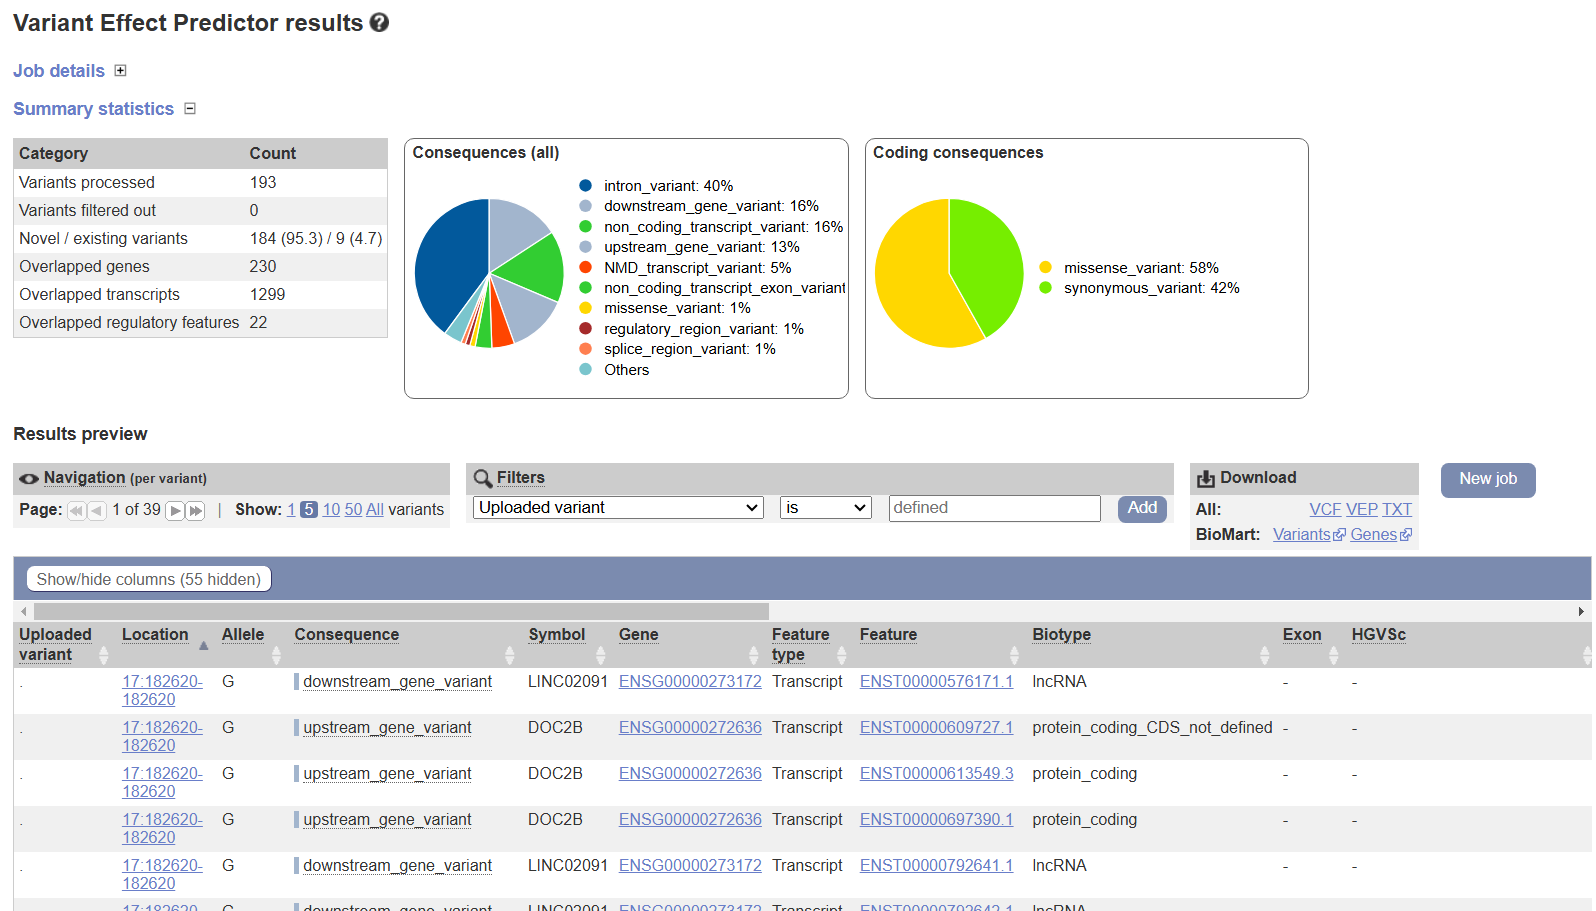
\includegraphics[width = \textwidth]{figs/vep-result.png}
\end{figure}

Para priorizar, se tendría en cuenta el score de AlphaMissense, SpliceAI, ClinPred, Revel, Sift y PolyPhen, buscando un consenso entre todos. Además, se puede buscar el identificador en ClinVar por si se hubiese recogido una asociación.